\documentclass[10pt]{article}

\usepackage{aas_macros}
\usepackage{graphicx}
\usepackage{subfigure}
\usepackage{fancyhdr}
\usepackage{amssymb,amsmath}
\usepackage{nicefrac}
\usepackage[usenames,dvipsnames]{color}
\usepackage[colorlinks,citecolor=RedViolet,urlcolor=blue]{hyperref}
\usepackage{doi}
\usepackage{setspace}
\usepackage[paperwidth=8.5in, paperheight=11in,top=2in, bottom=1.5in, left=1.2in, right=1.2in]{geometry}

\usepackage[authoryear,square]{natbib}
\pagestyle{fancy}



\fancyhead[R]{Veibell \thepage}
\fancyhead[L]{}

\def\titlepage#1#2#3#4#5#6{
 \begin{singlespace}
 \hbox{ }
 \begin{center}

  {\Large\bf #1 \mbox{}} \\

  \vfill
  by \\
  \vspace{2ex} % ex is the height of the lowercase 'x' for the current font. -jg
  #2 \\
  \vfill
   Submitted in partial fulfillment \\
   of the requirements for the degree of \\
   #3 \\
   (#4) \\
   George Mason University \\
   #5 \\
 \end{center}
 \vfill
  Doctoral Committee: \\[2ex]
  \mbox{ }\hspace{0.6in}
  \parbox{5.3in}{#6}
 \end{singlespace}
}

\begin{document}




\titlepage{PhD Dissertation Proposal}{Victoir Veibell}{Doctor of Philosophy}{School of Physics, Astronomy, and Computational Sciences}{2013}
{Dr. Robert Weigel, Chair\\ 
Dr. Kirk Borne\\
Dr. Fernando Camelli\\
Dr. Jie Zhang\\
}

\hrule
\setlength{\parskip}{3ex}
\renewcommand{\labelitemi}{$-$}

\newpage
\section{Abstract}

This dissertation intends to first: be a survey of current forecasting capabilities of statistical and  magnetohydrodynamic (MHD) methods of Earth's magnetosphere and the solar wind flow through interplanetary space, and second: attempt to improve upon forecasting methods by investigating the usefulness of various new models on both real and modeled data. The forecasting will be separated into two parts: that focusing on rare, but significant events (e.g. geomagnetic storms), and that focusing on general day-to-day predictions. It will encompass three main methods of forecasting: impulse response functions (IRF), nonlinear methods, and hybrid statistical methods that mimic MHD-modeling.

\section{Introduction}

The dynamic processes of Earth's magnetosphere and their various impacts on the planet and its inhabitants have been studied for centuries: from Celsius and Hiorter who noted a correlation between compass orientation and aurora \citep{Maunder} , to studies of The Carrington Event \citep{Carrington}, to Chapman and Ferraro's "A new theory of magnetic storms" \citep{Chapman}, scientists have been measuring the currents induced by the magnetosphere and trying to explain the effects they saw. With the advent of space flight, measurements of the magnetosphere in situ became possible and long-term data collection became prevalent, allowing for forecasting to become a feasible concept. Our current computational technology, combined with over 50 years' worth of satellite and ground based measurements \citep{HistMagnetometer}, allows for a much stronger statistics-based forecasting method to be performed and long-term analyses of the capabilities of computationally intensive forecasting methods.

Geomagnetic storms occur when the solar wind interacts with the Earth's magnetosphere in such a way as to produce significant disruptions in its normal, quiet-time, behavior. It is generally defined by a significant change to the magnetic field measured by multiple ground-based magnetometer measurements from stations spread around the world, in the case of the $K_P$ index, or around the geomagnetic equator in the case of the Disturbance storm-time ($D_{st}$) index. By using these indices, storms can be classified into categories of severity \citep{NOAAScale}. The definition of storms in the literature varies slightly between authors \citep{Yermolaev}, but most agree that sustained and abnormally perturbed near-earth magnetic field strengths over several hours or more constitutes a storm \citep{StormDefinition}. 

Geomagnetic storms can have significant impacts on Earth and space systems, from inducing currents in large power grids to harming satellite circuitry and onboard data \citep{1989Storm}. Because of the potential damage of such events, any ability to forecast a storm could allow operators to prevent or mitigate problems in their systems. Becuase of the large correlation of CMEs with geomagnetic storms \citep{Yermolaev}, it can be estimated that our forewarning time is the difference between observing a CME (via visual or X-ray methods) and its propagation time plus magnetospheric interaction time. This time can be anywhere from one to five days, depending on the speed of the CME and how it interacts with the interplanetary medium \citep{StormSources}. With a light delay of only eight minutes, this is ample time to see a storm approaching Earth and for operators to react, but a problem lies in the fact that storms are poorly predicted with such lead times\cite{WeigelDecisionTheory}. Some storms have slow onsets, some spike suddenly; some have high velocities, and some coincide with large amounts of high-energy particles; no single factor has yet proven to be a good predictor for storms, and while prediction has gradually improved over the years, there remains room for further study. 

Initial forecasts were based on an observed time delay between sunspots and geomagnetic storms \citep{SunspotStorms}. It then advanced to a basic theory involving electromagnetic interactions in the magnetosphere \citep{Chapman}. There now exist entire services dedicated to executing MHD-based models of the magnetosphere \citep{CCMC}, as well as multi-year, multi-institution efforts to survey the general statistics of modeling and forecasting of extreme events \citep{ExtremeEvents}.

The convergence of the advancement in both statistical and MHD-based simulation has led to a situation where the scientific community has the capacity for monitoring space weather in real time, and forecasting the Earth-side effects as the weather propagates past satellites.  There have been efforts to test the forecast performance of select models over a small number of geomagnetic events \citep{ANNforecast,StormModel,StatCompStorms,Yermolaev}. However no research has been done that involves the analysis of long-term forecasting performance of these models and comparison of the results with existing methods.

In order to effectively propose a research topic, the current limits of knowledge in the field must be mapped out. This includes current numerical methods being used for forecasts, current thoughts on the best types of models for the relevant systems, and what simulations have recently been conducted as well as any details they may have left out.

There has recently been some work in the following areas:
\begin{itemize} 
\item A large review of the general statistics and prediction of extreme events \citep{ExtremeEvents}
\item Modeling the frequency of strong storms using a power law model \citep{PowerLaw}
\item New GOES satellites with magnetometers to broaden overall measurement capabilities \citep{NewGOES}
\item Improvements to some of the standard physical models of the magnetosphere along with a software framework to couple multiple models into an adaptive model \citep{SWMF}
\item A physical model for forecasts in the radiation belt to protect satellites \citep{RadBeltForecast}
\item Models comparing seasonal variation in the coupled ionosphere-magnetosphere between numerical models and measurements \citep{Seasons}
\item A proof-of-concept paper modeling magnetic field variations with a solar wind driver \citep{DOYvar}
\end{itemize}


\section{Methods}
\subsection{Impulse Response}
Impulse response systems are systems in which the output (a response) is driven by an input (a series of impulses). A simple example would be making a loud noise in a concert hall. The response will be the unique echoes and reverberations created by the initial driving sound, and with enough noises, a statistical model can be generated that will map the input sound to a response echo. In the magnetosphere, the most used example is an impulse of $v_{B_s}$ driving the Auroral Electrojet (AE/AL) index \citep{VBzAL}, or the Disturbance Storm Time ($D_{st}$) index \citep{VBzDST}, also shown in Figure \ref{VBzIRplot}.

\begin{figure}[htp]
\centering
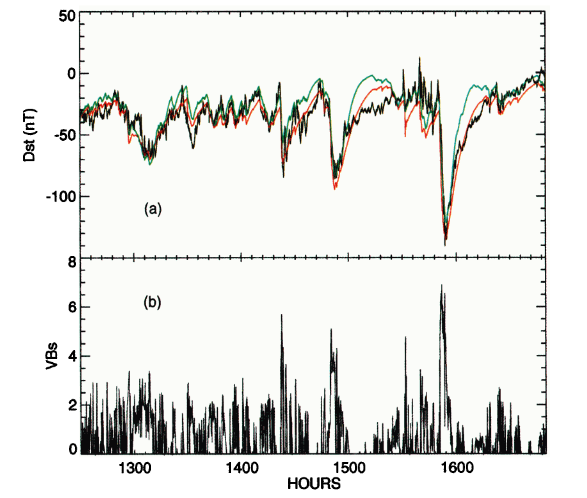
\includegraphics[scale=0.40]{VBzIR.png}
\caption{DST (black), nonlinear ARX model (red), Burton et al 1975 model (green). (b) $v_{B_S}$ impulse.\citep{ARXEqn}}
\label{VBzIRplot}
\end{figure}

This plot shows how different models are used to try to predict magnetospheric variables with varying amounts of success. In this proposal, what starts as a simple Box-Jenkins model of the form \citep{DOYvar}:
\begin{align*}
x(t)&=c+\sum_{j=0}^{m}{a_j f(t-j\Delta t)}
\end{align*}
can be modfied with an auto-regressive component to be an autoregressive model with exogenous inputs (ARX) such as that used in \citep{ARXEqn}, taking the form:
\begin{align}
\hat{x}(t+\Delta t)&=\sum_{i=0}^la_i\cdot x(t-i\Delta t)+\sum_{j=0}^m b_j\cdot f(t-j\Delta t)+c
\label{ARXEqn}
\end{align}
Where $m$ and $l$ are the number of coefficients desired for including previous data points in the prediction, and $c$ is a factor to remove the mean offset from the data. Also worth noting: in some cases the starting value of the iterators can be individually increased if there is a known delay in response time or there is a desire to predict further into the future. In the sampled paper \citep{ARXEqn}, second order equations ($m=2$) were used with anywhere from one to four driving coefficients, but in practice any number of coefficients and any number of driving variables can be used up to some fraction of the number of data points that allows the coefficient matrices to still be solved. 

That said, there generally is a limit to the usefulness of large-lag data \citep{ExtremeEvents}. By looking at a plot of the cross correlation relative to the number of coefficients, a limit will generally be seen where overspecification of the system (by adding more coefficients) is no longer helpful. By creating a threshhold of change in fit per coefficient added (perhaps via a bootstrap method), the minimum number of coefficients needed to optimally model the system can be determined.

By constructing a linear system of equations from Equation \ref{ARXEqn}, the coefficients can be solved for in a general matrix form (where, in this case, $l=m$):
\[
\left( \begin{array}{ccccccc}
x_0 & ... & x_{l-1} & f_0 & ... & f_{l-1} & 1\\
x_1 &     & x_l & f_l &  &f_l & 1\\
... &     &     &     &  &   & \\
x_{N-l} & ... & x_{N-1} & f_{N-l} & ... & f_{N-1} & 1
\end{array} \right)
\left(\begin{array}{c}
a_0\\...\\a_{l-1}\\b_0\\...\\b_{l-1}\\c
\end{array}\right)
=
\left(
\begin{array}{c}
x_l \\ x_{l+1} \\ ... \\ x_{N}
\end{array}
\right)
\]

This is a very simple model for the behavior of a system. However, it has been shown that the set of coefficients describing the response of a system can change with storm intensity \citep{ARXEqn}, the time scale modeled \citep{Coupling}, and even the time of day \citep{VBzAL}. This creates a very large number of possible directions for research, from trying to predict storm onsets, to trying to predict storm intensities, to trying to model the overall shape and behavior of a storm, as well as all of the other possible interactions outside of storm-time. 

\subsection{Caveats}
There are a number of things that, ideally, must come together to make this kind of data prediction work. For one: ARX methods can often be heavily dependent on a concept known as "persistence", whereby the best prediction for a variable at any time is that same variable at the last measured time step. For example, if the high temperature today is $70^\circ$, it is fairly likely that the high temperature tomorrow will be near $70^\circ$. Too much reliance on persistence forecasting, though, and predictions can lose their usefulness. Figure \ref{persist}, for example, shows how a model can achieve high correlation with persistence, but be almost entirely useless for predicting events before they happen:

\begin{figure}[h!]
\centering
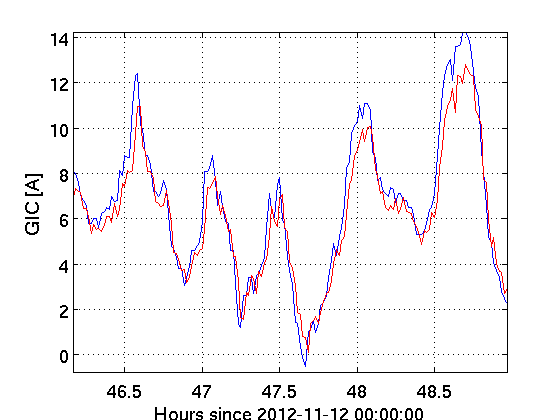
\includegraphics[scale=0.45]{GICshift.png}
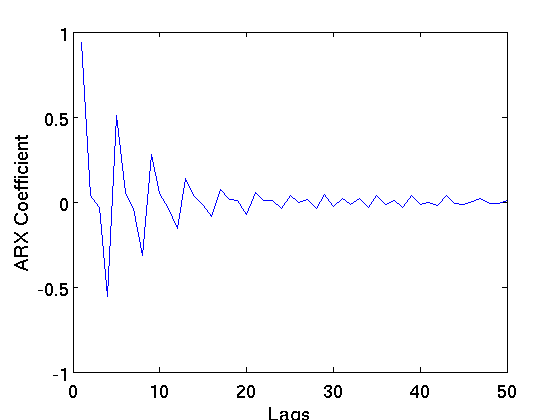
\includegraphics[scale=0.45]{GICCoef.png}
\caption{Persistence forecast; model in red}
\label{persist}
\end{figure}

In this case, it is clear that the biggest auto-correlation coefficient comes at 1 time lag, meaning the most recent measurement has the most weight in a forecast. For day-to-day behavior, this is acceptable as being part of the behavior of the system. For the forecasting of extreme events, however, another metric must be used that measures the ability of the model to predict events at or before their actual occurrence, while simultaneously avoiding predicting events that do not happen. One method for comparing models in this fashion is by using the Heidke Skill Score \citep{Heidke,Brier}:
\begin{align*}
S=\frac{R-E}{T-E}
\end{align*}
Where $R$ is the number of correct forecasts, $T$ is the total number of forecasts, and $E$ is the number expected to be correct by, in this case, a persistence forecast. This can be adapted to either consider a range of "correctness", or a binary threshold to be met. It may be desired to assign a cost-weighting to success rates one way or another. If, say, it costs \$1 million to prepare a power grid for a storm, 10 false alarms to every one storm gets costly unless successfully preparing for that one storm saves \$1 billion. To do this, a simple algorithm for the utility of a forecast can be used \citep{WeigelDecision}:
\begin{align*}
U_F\equiv BN_H-CN_{\bar{H}}>0
\end{align*}
Where $N_H$ is the number of correct forecasts, $N_{\bar{H}}$ is the number of false alarms, $C$ is the cost of taking mitigating action, and $B$ is the benefit from correctly taking mitigating action. This method has caveats discussed in \citep{WeigelDecision}, but is a good metric for forecast utility when costs are known, and some measure of success can be determined. 

The other major problem in forecasting is that of lead time. Being able to forecast a storm one minute in advance will not help prevent much damage, so the sooner an accurate prediction can be made, the more useful it may be. Consider Figure \ref{Lags}:

\begin{figure}[h!]
\centering
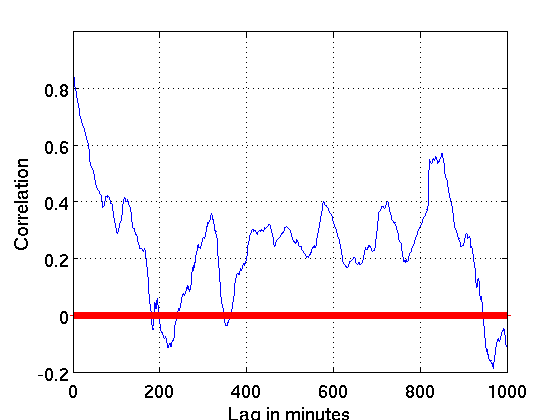
\includegraphics[scale=0.50]{GIClags.png}
\caption{Correlation vs lags}
\label{Lags}
\end{figure}

In this figure, a set of predictions for ground-induced current (GIC) were made further and further from the current magnetic field and GIC measurements. While an accurate prediction can be made one minute in advance, a prediction 3 hours in advance has almost no correlation with what actually happens. This is the main problem that this dissertation hopes to address.


\subsection{Nonlinear approaches}
Other models will be devised to test nonlinear approaches to forecasting. One popular choice is models based on neural networks \citep{NNARMA,ANNforecast} which allow for adaptive weights and a model that can approximate a non-linear system. The usefulness of this is apparent in a few key points: the weights of contribution of any particular variable to a system will likely be nonlinear in some fashion (e.g. a ground station's measurements will depend on sunlight heating the ionosphere which depends on latitude, time of year, and time of day), and allowing for the non-linear effects of saturation where perhaps the magnetosphere will behave differently after reaching certain levels of particle density or electric potential.

Another algorithm known as Principal Component Analysis can be used to take the large number of possible variables and define an orthogonal set of vectors that most efficiently encapsulate the variance in the data. By doing this, the number of variables needed for computing any linear or non-linear algorithm can be reduced and optimized, making predictions quicker while maintaining most of the predictive benefits of using all possible data.


\section{Proposal}

Two main avenues are to be explored with this dissertation: that of finding where, exactly, the impulse response prediction methods fit within known forecasting techniques, and that of improving the forecasts in areas where it is already known to work. By approaching the forecasting models from a few different directions, improvements can be made in predicting space weather allowing for both an expanded scientific knowledge base, and be an aid to forecasters.

\subsection{Hybrid model approach}
Since the speed of this method is essentially just that of building and solving an overdetermined system of equations, a problem that has been very highly optimized \citep{LP}, it is much faster than any models based on physical solutions of the MHD equations. Since these optimized solution methods are built into most modern languages and common libraries, the code base also comes with low overhead. This should make a simple task of testing the hypothesis that impulse response methods can, in some way, replace or augment complex physical models for very quick forecasts instead of needing days to run a simulation. Whether this is feasible or not, and if so, in which cases it would be feasible, would be the subject of study.

By taking an MHD model from the Community Coordinate Modeling Center \citep{CCMC} such as BATS-R-US and inputting solar wind conditions from an observed time period, an autoregressive moving average (ARMA) model can be generated that takes two timeseries: one of the empirical measurements, and one of the MHD model's next output state variables using those measurements. The combination of the two can generate a set of statistical model coefficients that will, hopefully, model the model.

\subsection{Characterizing system}
The other major task this dissertation aims to address is that of characterizing the magnetosphere-ionosphere system in terms of an impulse response model. While some relations are known to be easily forecastable in this way, the prospect does not seem to have been explored fully. If it turned out that some important variable, say mass density in the magnetosphere, was forecastable as a response to some as-of-yet unthought-of impulse, like say, number of sunspots, not only would this improve forecasts, but would also lead to new research on the coupling of the two variables.

It is also possible to, in a way, characterize the coupling of a system by working backwards from the statistically determined impulse response coefficients. If the system of equations is told to produce 10 coefficients, but only comes back with one significant one that does a reasonable job of forecasting, it can be presumed the relationship is linear. By taking a large set of variables \citep{Denton} and attempting various combinations of forecasts to find effective predictors, perhaps some new avenue of research can be developed, and if not, then at least the magnetosphere can be said to not be so simply coupled in any way. 

\subsection{Increasing lead times}
Ideally, since the current lead time of storm predictions from $B_S$ is under an hour \citep{StatCompStorms}, some method can be found to allow accurate forecasting of a storm earlier. Whether this method relies on an as-yet undiscovered ARX coupling, or some other statistical use of known variables, is something this dissertation hopes to explore. However, one notable trait of a system that allows for useful forecasting is one in which a time lag will not inhibit a forecast. If an IRF model can be developed in which the response can be modeled from a much earlier impulse, a forecast can be made that much sooner. For example, the often-modeled $D_{ST}$ index can be almost as well forecasted without persistent knowledge as with it, as seen in Figure \ref{DST}.

\begin{figure}[h!]
\centering
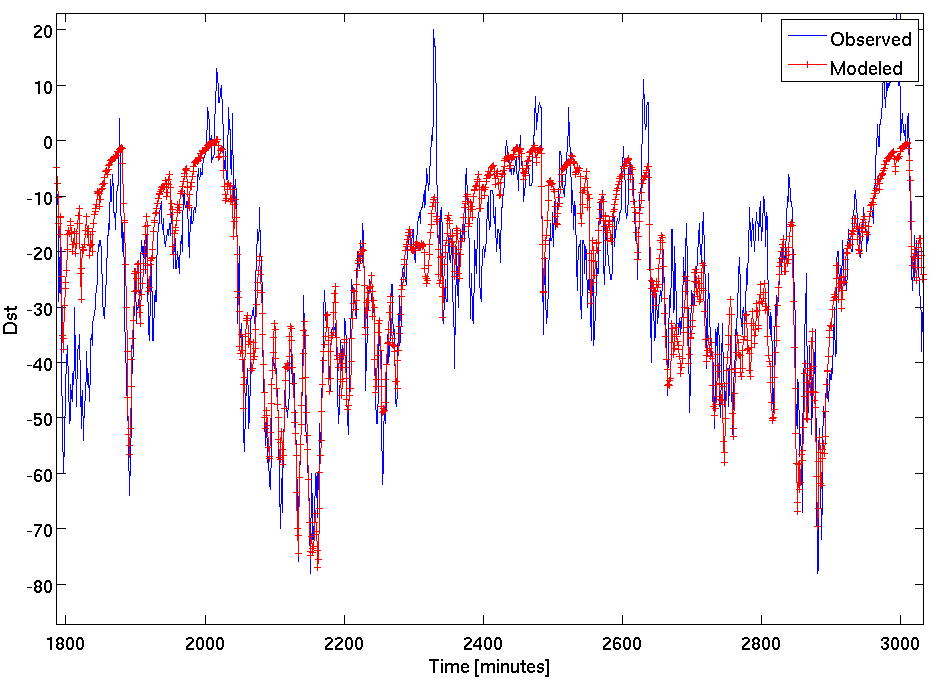
\includegraphics[scale=0.25]{DstExample.png}
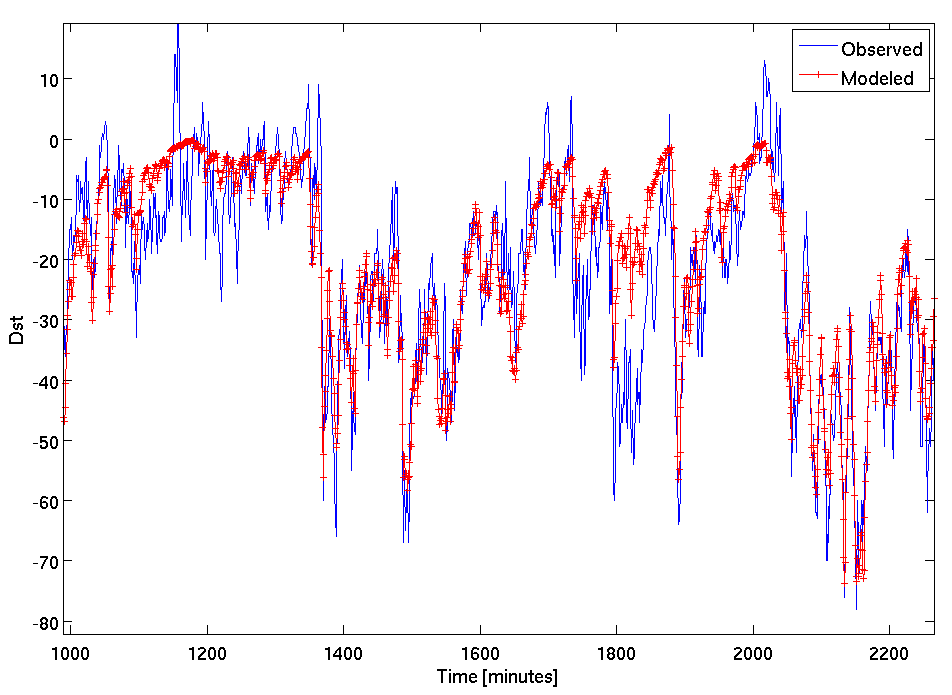
\includegraphics[scale=0.25]{DstNoPersist.png}
\caption{Dst with and without persistence}
\label{DST}
\end{figure}

The significance is that, in a case such as this, the forecast can be made from an impulse as it propagates through space long before it interacts with Earth, giving that extra lead-time to prepare for any potential impacts. 

In order to start testing this, a large set of variables will be taken \citep{Denton}, and an automated system will attempt to predict common state variables (velocity, magnetic field, pressure, density, etc) from all of the database variables. The optimum number of variables will be tested in the manner outlined previously to find if any time lag exists in some correlations. From there, combinations of variables as inputs will be tested up to the computational limits of the machine (noted because a prior attempt to create a model with 78 multi-year-long impulses for one output far exceeded the memory limits of the testing machine). If, at that point, no other promising avenues of study have arisen, this research will expand on other known linear models, followed by attempts at prediction using nonlinear models.

The major constraint of this study is time, and the fact that not every avenue can be explored. The dissertation will tend to focus on extreme events, and on the impacts of these events on ground-based systems, but as time permits it will branch out into a wider scope of analysis.


\footnotesize
\bibliographystyle{vplainnat}

\bibliography{reportbib}


\section{Things to add}
\begin{itemize}
\item Proofs of statistical validity? (time-stationarity, optimal solution to LSEs, etc)
\item More on ground based measurements and interpolation

\end{itemize}


\end{document}